\documentclass[a4paper,10pt]{article}
\usepackage[utf8]{inputenc}
\usepackage[english]{babel}
\usepackage{geometry}
\usepackage{graphicx}
\usepackage{blindtext}
\usepackage{titling}
\usepackage[nottoc]{tocbibind} %Adds "References" to the table of contents
\usepackage{fontawesome}
\usepackage{url}
\usepackage{hyperref}
\usepackage{float}
\usepackage{subcaption}
\usepackage{color}
\usepackage{graphicx}
\graphicspath{ {./img/} }
\hypersetup{
	colorlinks=true,
	linkcolor=black,
	filecolor=magenta,      
	urlcolor=blue,
}
\usepackage{listings}



\newcommand{\github}[2][13pt]{\hspace{5pt}\faGithub\hspace{5pt}\fontsize{#1}{0}\url{#2}}

%Document title, author and date (empty)
\title{Game of Life}
\author{Francesco Corti - 606922}
\date{April 2020}

% Definition of \maketitle
\makeatletter         
\def\@maketitle{
	\raggedright
	%\includegraphics[width = 40mm]{logo.jpg}\\[8ex]
	\begin{center}
		{\Huge \bfseries \sffamily \@title }\\[4ex] 
		{\Large  \@author}\\[4ex] 
		\@date\\[8ex]
		
\includegraphics[scale = 0.35]{logo-Pisa.jpeg}
\end{center}}
\makeatother

%Beginning of the document
\begin{document}
		\maketitle
		\begin{abstract}
			The purpose of the assignment was to implement different versions of Game Of Life, a game devised by the British mathematician John Horton Conway in 1970.
			Three versions were developed: sequential, parallel using C++ threads version and parallel using OpenMP. 
		\end{abstract}
\vspace{0.3cm}

\section{Code structure}
The program has a single class \textit{gameOfLife.h} that expose three public methods \textit{Sequential}, \textit{StandardThreads} and \textit{OpenMP}. The user needs to pass from the command line the following parameters: number of iteration, random number generator seed, the dimension of the board and the parallelism degree. By default the program computes the sequential version followed by the Fork-Join and the OpenMP. For each version the time spent on computing is printed out on the screen.

In order to provide an efficient implementation the two-dimensional board is saved as one-dimensional \textit{bool*} array, all the index are adjusted to make the computation correctly. After each iteration the update version of the board is swapped using the \textit{std::swap} method. This operation prevents a total copy of the matrix and lets the system scale well even with a large matrix. All the code written is hosted on a public repository named \href{https://github.com/FraCorti/PSD-Assignments}{PSD-Assignments} in GitHub.

\section{Measures}
To understand the performance of the program two metrics related to performance and parallelism, \textit{speedup} and \textit{scalability}, were used as performance indicators. For these metrics the speedup asymptote is given by $f(n) = n $. 
\subsection{Speedup}
The \textit{speedup} is the ratio between the best known sequential execution time and the parallel execution time. This is obtained by the formula:
\begin{equation}
\textnormal{s(n)} = \frac{T_{seq}}{T_{par}(n)}
\end{equation}
 and gives a measure of how good is our parallelization with respect to the best sequential computation.
\subsection{Scalability}
The \textit{scalability} is the ratio between the parallel execution with parallelism degree equal to 1 and the parallel execution with parallelism degree equal to \textit{n}. This is obtained by the formula:
\begin{equation}
\textnormal{scalab(n)} = \frac{T_{par}(1)}{T_{par}(n)}
\end{equation}
and measures how efficient is the parallel implementation in obtaining better performance on bigger parallelism degree.
\section{Results}
I initially developed a sequential implementation of the program as a baseline. This was done to save the sequential time $T_{seq}$ that was used to compute the speedup curves. After that I developed the parallel version with C++ threads (only) and OpenMP, for each of them I saved $T_{par}(1)$ which is the parallel execution time with parallel degree equal to 1 that was used to compute the scalability curves. 

To obtain good results the program was tested in the Xeon PHI with the board's dimensions of 500x500, 5000x5000 and 10000x10000. For each of these dimensions the zoomed plot is shown on the right side. 



\subsection{Speedup curves}


\begin{figure}[H]
	\centering
	\begin{minipage}[t]{0.55\linewidth}
		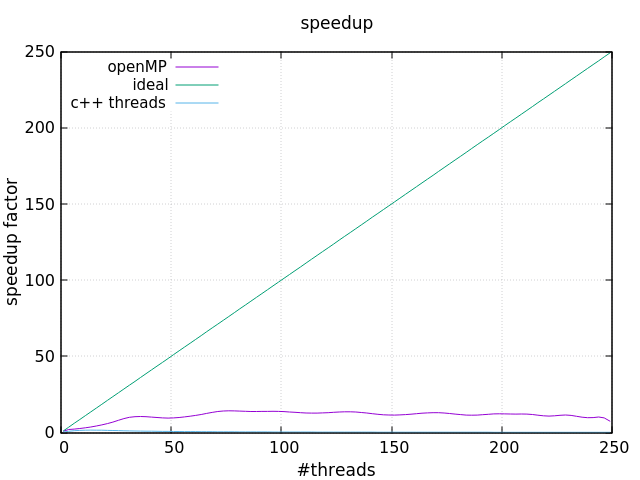
\includegraphics[width=\linewidth]{500_standard_speed.png}
		%\subcaption{MSE}
	\end{minipage}%
	\begin{minipage}[t]{0.55\linewidth}
		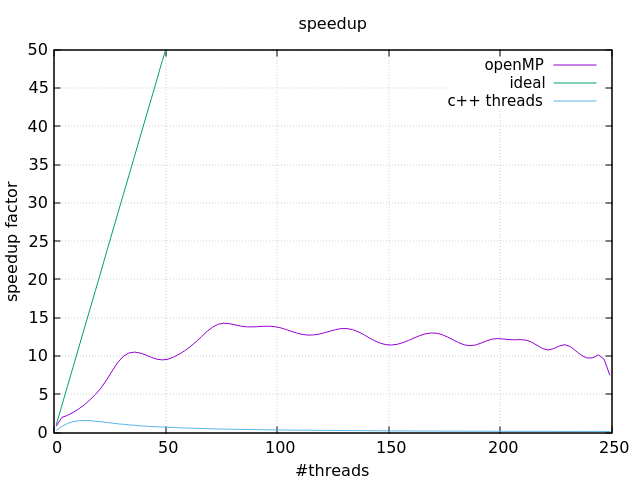
\includegraphics[width=\linewidth]{500_zoomed_speed.png}
		%\subcaption{Accuracy}
	\end{minipage}
	\caption{Speedup 500x500 boards.}
	\label{500Speed}
\end{figure}

\begin{figure}[H]
	\centering
	\begin{minipage}[t]{0.55\linewidth}
		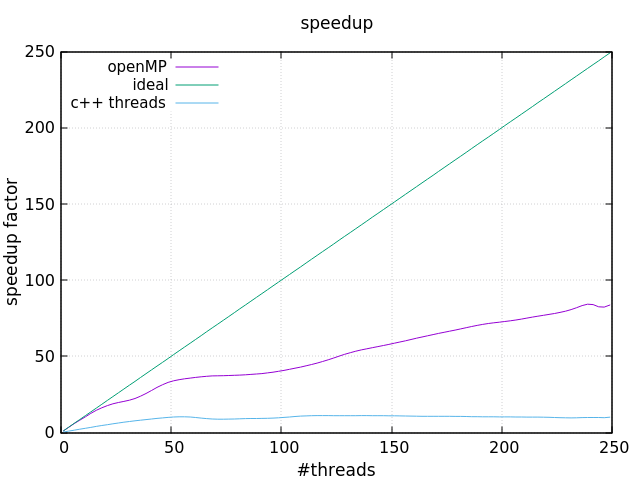
\includegraphics[width=\linewidth]{5000_standard_speed.png}
	\end{minipage}%
	\begin{minipage}[t]{0.55\linewidth}
		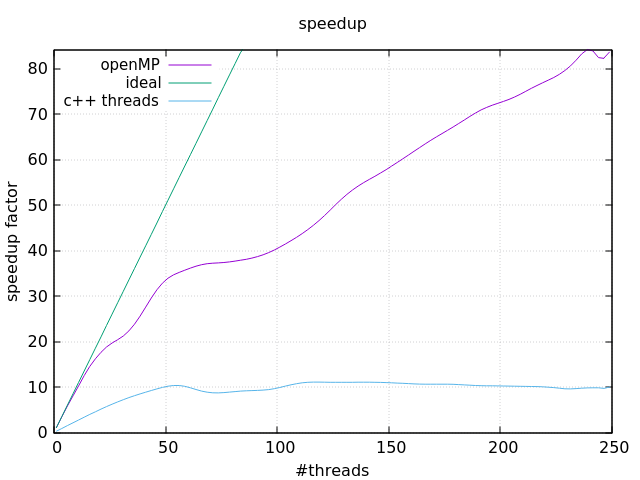
\includegraphics[width=\linewidth]{5000_zoomed_speed.png}
	\end{minipage}
	\caption{Speedup 5000x5000 boards.}
	\label{50000Speed}
\end{figure}

\begin{figure}[H]
	\centering
	\begin{minipage}[t]{0.55\linewidth}
		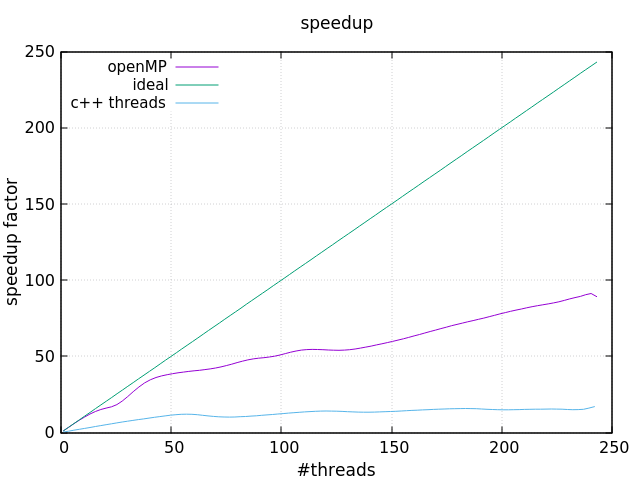
\includegraphics[width=\linewidth]{10000_standard_speed.png}
		%\subcaption{MSE}
	\end{minipage}%
	\begin{minipage}[t]{0.55\linewidth}
		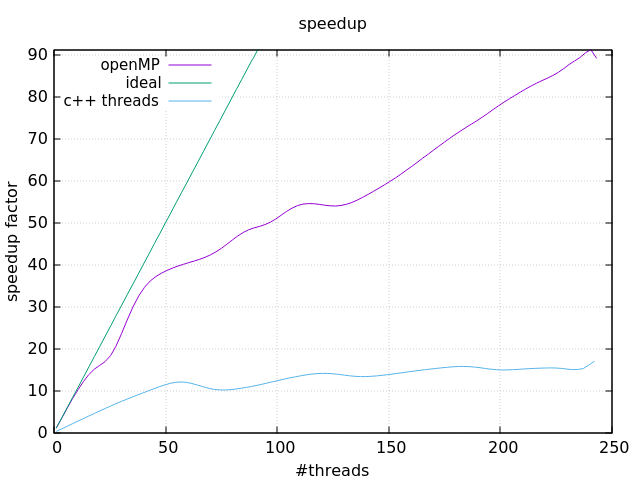
\includegraphics[width=\linewidth]{10000_zoomed_speed.png}
		%\subcaption{Accuracy}
	\end{minipage}
	\caption{Speedup 10000x10000 boards.}
	\label{10000Speed}
\end{figure}

\subsection{Scalability curves}
\begin{figure}[H]
	\centering
	\begin{minipage}[t]{0.55\linewidth}
		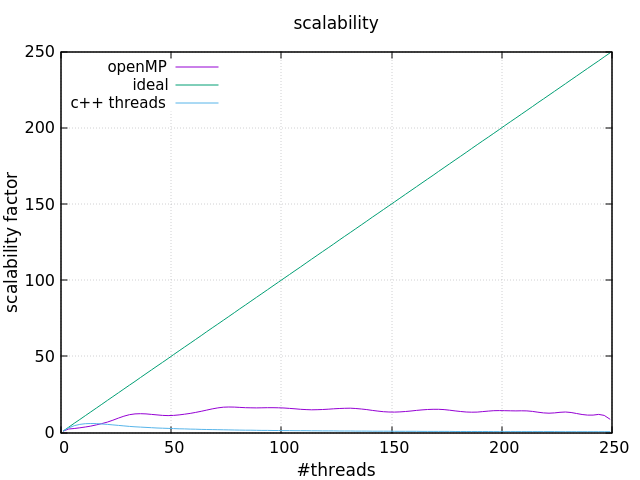
\includegraphics[width=\linewidth]{500_standard_scal.png}
		%\subcaption{MSE}
	\end{minipage}%
	\begin{minipage}[t]{0.55\linewidth}
		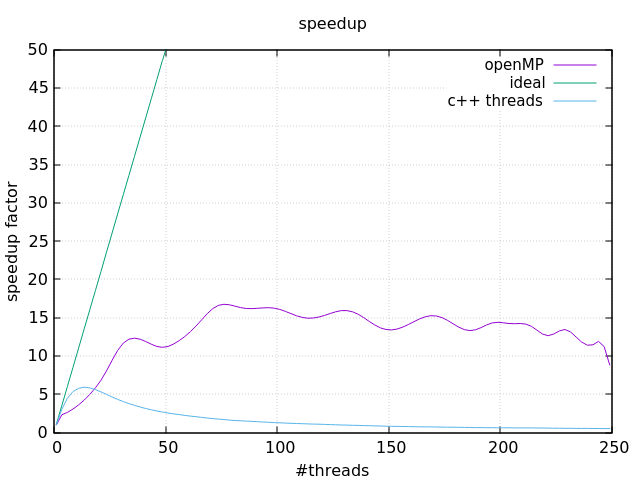
\includegraphics[width=\linewidth]{500_zoomed_scal.png}
		%\subcaption{Accuracy}
	\end{minipage}
	\caption{Scalability 500x500 boards.}
	\label{500Scal}
\end{figure}

\begin{figure}[H]
	\centering
	\begin{minipage}[t]{0.55\linewidth}
		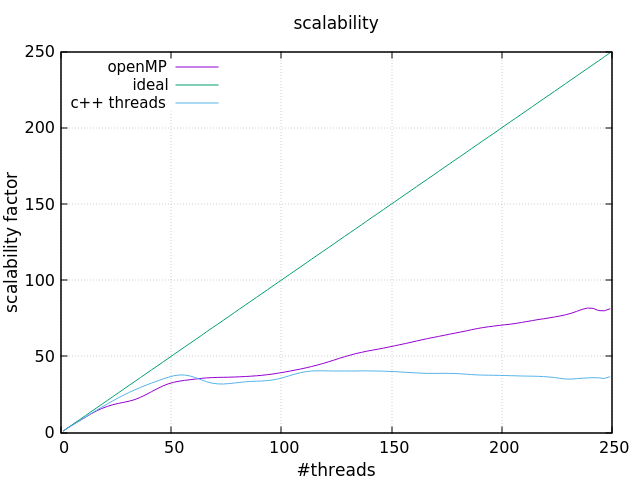
\includegraphics[width=\linewidth]{5000_standard_scal.png}
		%\subcaption{MSE}
	\end{minipage}%
	\begin{minipage}[t]{0.55\linewidth}
		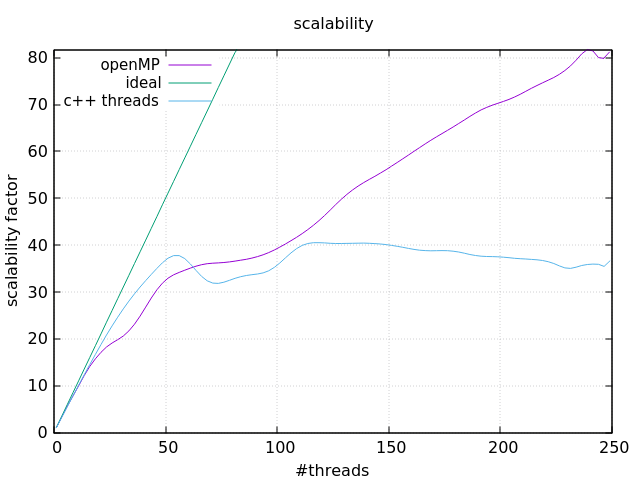
\includegraphics[width=\linewidth]{5000_zoomed_scal.png}
		%\subcaption{Accuracy}
	\end{minipage}
	\caption{Scalability 5000x5000 boards.}
	\label{50000Scal}
\end{figure}

\begin{figure}[H]
	\centering
	\begin{minipage}[t]{0.55\linewidth}
		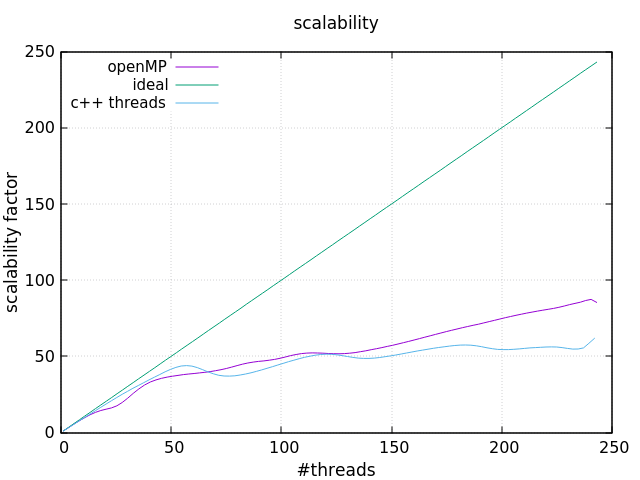
\includegraphics[width=\linewidth]{10000_standard_scal.png}
		%\subcaption{MSE}
	\end{minipage}%
	\begin{minipage}[t]{0.55\linewidth}
		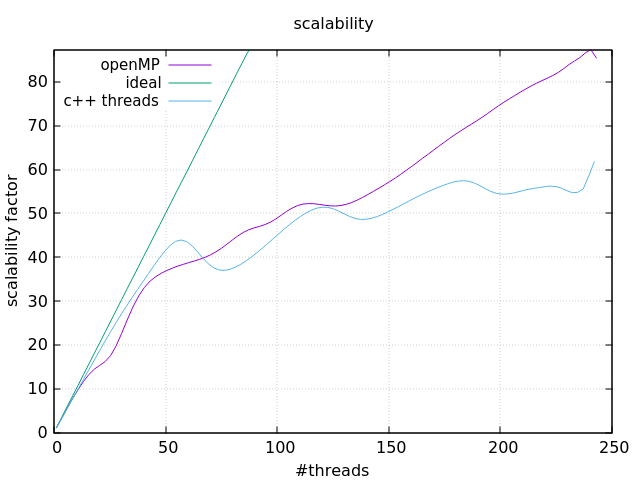
\includegraphics[width=\linewidth]{10000_zoomed_scal.png}
		%\subcaption{Accuracy}
	\end{minipage}
	\caption{Scalability 10000x10000 boards.}
	\label{10000Scal}
\end{figure}

\section{Conclusion}
As we can see in figure \ref{500Speed} not all the computations can benefit of an high parallelism degree, with small boards and a high parallelism degree the benefits of adding threads doesn't speed up the computation time obtained to solve the problem. This because the \textit{overhead} taken to set up the parallel computation can exceed the computing time taken to solve the problem and the amount of work given to the worker isn't enough to justify the time spent to spawn them. 

Game of Life with little board dimensions isn't a heavy problem to compute, however if we expand the dimensions we can benefit from a high parallelism degree and obtain a good speedup (nearly sublinear with OpenMP) due to parallel computation, see figure \ref{10000Speed}. 

\end{document}
